%\documentclass[10pt,xcolor=dvipsnames,flushleft]{beamer}

\usetheme{guadec}
%\usecolortheme[named=Red]{structure}
\usepackage[utf8]{inputenc}
\usepackage[T1]{fontenc}
\usepackage[italian]{babel}
\usepackage{graphicx}
\usepackage{lipsum}
\usepackage[makeroom]{cancel}
%\makeatother
%\setbeamertemplate{footline}
%{
%  \leavevmode%
%  \hbox{%
%  \begin{beamercolorbox}[wd=.4\paperwidth,ht=2.25ex,dp=1ex,center]{author in head/foot}%
%    \usebeamerfont{author in head/foot}\insertshortauthor
%  \end{beamercolorbox}%
%  \begin{beamercolorbox}[wd=.6\paperwidth,ht=2.25ex,dp=1ex,center]{title in head/foot}%
%    \usebeamerfont{title in head/foot}\insertshorttitle\hspace*{3em}
%    \insertframenumber{} / \inserttotalframenumber\hspace*{1ex}
%  \end{beamercolorbox}}%
%  \vskip0pt%
%}

\usepackage{color}	
\usepackage{tikz, pgfplots}
\usepackage{circuitikz}
\usetikzlibrary{positioning}
\usepackage{pstricks}
\usepackage{pgfplots}
\usetikzlibrary{arrows,shapes}
\usetikzlibrary{decorations.pathmorphing}
\usetikzlibrary{decorations.markings}



\makeatletter
\setbeamertemplate{navigation symbols}{}
%\setbeamertemplate{footline}[frame number]{}
\useinnertheme[shadow=true]{rounded}
\setbeamersize{sidebar width left = 0mm}
\setbeamersize{sidebar width right = 0mm}
%\setbeamercolor{title}{fg=blue!70!black,bg=blue!10!white}
\linespread{0.9}


\newcommand{\tit}{\usebeamercolor[fg]{titlelike}}
\renewcommand{\gray}{\color{black!55}}
\newcommand{\omissis}{[\textellipsis\unkern]}

\newcommand*{\TakeFourierOrnament}[1]{{%
\fontencoding{U}\fontfamily{futs}\selectfont\char#1}}
\newcommand*{\danger}{\TakeFourierOrnament{66}}

\tikzset{>=latex}
\tikzset{
    field1/.style={draw=red, postaction={decorate},
        decoration={markings,mark=at position .55 with {\arrow[red]{>}}}}}
\tikzset{
    field2/.style={draw=black, postaction={decorate},
        decoration={markings,mark=at position .55 with {\arrow[black]{>}}}}  }


\AtBeginSection[]
{
  \begin{frame}{Indice}
    \tableofcontents[currentsection]
  \end{frame}
}

\setbeamercovered{transparent}

\title{Big Data in Streaming}
\subtitle{elaborazioni e visualizzazione in Real Time}
\author{Davide Vergari aka OutOfBounds \\ \& \\Davide Isoardi aka Abacus}
\date{22 Ottobre 2016}
\institute{Linux Day 2016}



\begin{document}
	%\beamertemplateshadingbackground{white!100!}{gray!30}


\begin{frame}
	\maketitle
	\begin{center}
		
\includegraphics[scale=0.45]{img/cc-nc-sa}
	\end{center}

\end{frame}



%\begin{frame}{Indice}
%\tableofcontents
%\end{frame}



%\section{Contestualizzazione}
%\subsection{Dove e Quando}
%\subsection{Bisogni Educativi Speciali}
%\subsection{Indicazioni Nazionali}
%\subsection{Metodologie e strumenti}
%\subsection{Il ruolo del docente}









\begin{frame}
\frametitle{Big Data e il V.V.V.}
\framesubtitle{Cosa sono?}

	\begin{columns}
		\column{0.8\textwidth}
		\begin{block}{}
		\begin{center} \textbf{\tit Volume: } peta e peta di dati distribuiti \end{center}
		\end{block}
	\end{columns}	

	\begin{columns}
		\column{0.8\textwidth}
		\begin{block}{}
		\begin{center} \textbf{\tit Velocità: } flusso continuo da tanti (migliaia) device - \textbf{RealTime}\end{center}
		\end{block}
	\end{columns}
	
	\begin{columns}
		\column{0.8\textwidth}
		\begin{block}{}
		\begin{center} \textbf{\tit Varietà: } dati etereogenei non statici nel tempo\end{center}
		\end{block}
	\end{columns}

	\begin{columns}
		\column{0.8\textwidth}
		\begin{block}{}
		\begin{center} {\huge \tit \danger}  Avercelo grosso, il \textbf{DB}, non è sinonimo di BigData \end{center}

		\end{block}
	\end{columns}

\vspace{1cm}

\begin{center}
{\gray Quindi paralleliziamo le operazioni:\\ \textbf{Ingestion}, \textbf{I/O su file system}, \textbf{Elaborazione} }
\end{center}

\end{frame}

\begin{frame}[t]
\frametitle{L'ecosistema Hadoop}

\begin{block}{}
	\begin{center}
		\textit{Non è un tool, ma un insieme di service che completano la soluzione a seconda delle esigenze del business.}
	\end{center}
\end{block}

%\begin{block}<2->{Tante ``distribuzioni'', un solo padre}
%	\begin{center}
%		\begin{itemize}
%			\item Hortonworks
%			\item BigTop
%			\item Claudera
%			\item MapR
%		\end{itemize}
%	\end{center}
%\end{block}

\begin{columns}
	\begin{column}{0.5\textwidth}
		
\includegraphics[scale=0.4]{img/hws_logo}
	\end{column}
	\begin{column}{0.5\textwidth}
		
\includegraphics[scale=0.2]{img/cloudera_logo}
	\end{column}
\end{columns}
\begin{center}
	
\includegraphics[scale=0.2]{img/mapR_logo}
\end{center}

\end{frame}

\begin{frame}[t]
\frametitle{Hadoop - Da dove nasce}

\begin{center}
	
\includegraphics[scale=0.45]{img/solr-logo}\\
	
	
\includegraphics[scale=0.45]{img/nutch-logo}
\end{center}

\end{frame}

\begin{frame}[t]
\frametitle{Hortonworks Data Platform - dove siamo}

\begin{center}
	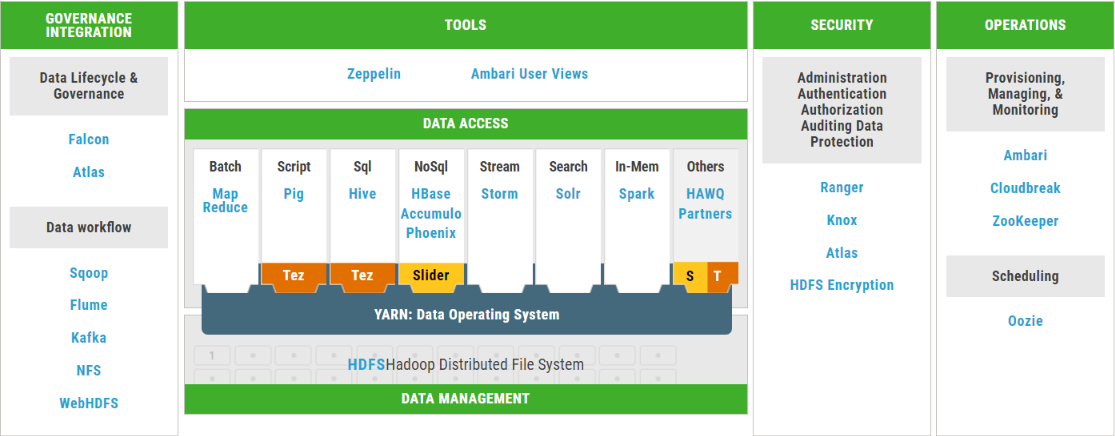
\includegraphics[scale=0.45]{img/HDP_25}
\end{center}

\end{frame}




\begin{frame}
\frametitle{Cosa vediamo oggi?}
\begin{columns}
	\begin{column}{0.5\textwidth}
		
\includegraphics[scale=0.4]{img/icon-hdf}
	\end{column}
	\begin{column}{0.5\textwidth}
		
\includegraphics[scale=0.2]{img/nifi-logo}\\
		
\includegraphics[scale=0.2]{img/kafka-logo}\\
		
\includegraphics[scale=0.2]{img/storm-logo}
	\end{column}
\end{columns}

\end{frame}

\begin{frame}
	\frametitle{Riferimenti}
	\begin{itemize}
		\item GitHub repo di Davide Isoardi \href{https://github.com/disoardi}{https://github.com/disoardi}
		\item GitHub repo di Davide Vergari \href{https://github.com/dvergari}{https://github.com/dvergari}
		\item GitHub repo di eCube s.r.l dove ci son le demo complete ed il processors NiFi per la sentiment analisys \href{https://github.com/ecubesrl}{https://github.com/ecubesrl}
	\end{itemize}
	\begin{block}{}
		\begin{center}
			Qui trovate a grandi linee i riferimenti della demo vista nel talk, ovviamente con alcune differenze e, soprattuto, replicabile su una singola macchina. Ad esempio la demo \href{https://github.com/ecubesrl/tweetsdemo-service}{tweetsdemo-service} è funzionante anche direttamente su una Sandbox (leggete il README)
		\end{center}
	\end{block}
	\begin{block}{eMail}
		\begin{center}
			Pre altre info contattatemi via mail all'indirizzo abacus@linux.it
		\end{center}
	\end{block}

\end{frame}




\end{document}
